\documentclass[11pt,largemargins]{homework}

% TODO: replace these with your information
\newcommand{\hwname}{Ally Smith}
\newcommand{\hwemail}{Section B}
\newcommand{\hwtype}{Homework}
\newcommand{\hwnum}{5}
\newcommand{\hwclass}{}
\newcommand{\hwlecture}{0}
\newcommand{\hwsection}{Z}

\begin{document}
\maketitle

% Your content
\question{Consider the following code:}

\begin{minipage}{\textwidth}
    \begin{minipage}{.4\textwidth}
        \begin{verbatim}
P1: {
    shared int x;
    x = 10;
    while (1) {
        x = x - 1;
        x = x + 1;
        if (x != 10) {
            printf("x is %d", x)
        }
    }
}
        \end{verbatim}
    \end{minipage}
    \hfill{}
    \begin{minipage}{.4\textwidth}
        \begin{verbatim}
P2: {
    shared int x;
    x = 10;
    while (1) {
        x = x - 1;
        x = x + 1;
        if (x != 10) {
            printf("x is %d", x)
        }
    }
}
        \end{verbatim}
    \end{minipage}
\end{minipage}
Note that the scheduler in a uni-processor system would implement
pseudo-parallel execution of these
two concurrent processes by interleaving their instructions, without
restriction on the order of the
interleaving.

\textbf{Show a sequence} (i.e., trace the sequence of interleavings of
statements) such that the statement
“x is 10” is printed.

\begin{minipage}{.4\textwidth}
    \begin{minipage}{.15\textwidth}
        \begin{verbatim}
x = 10;


x = x - 1;
x = x + 1;
if (x != 10)
printf("x is %d", x)
        \end{verbatim}
    \end{minipage}
    \hfill{}
    \begin{minipage}{.15\textwidth}
        \begin{verbatim}

x = 10;
x = x - 1;
            
            
            
            
        \end{verbatim}
    \end{minipage}
\end{minipage}

\clearpage
\question{Answer the following questions on deadlock:}
\begin{alphaparts}
    \questionpart{What are the necessary conditions for a deadlock?}

    Circular wait, no preemption, hold \& wait, and mutual exclusion.

    \questionpart{Describe the method to address the condition of hold and
        wait, and explain why it works.}

    To address this, you can require that a process request all of its required
    resources at one time and blocking the process until all requests can be
    granted simultaneously. This ensures that the program will not be waiting
    on anything before it actually starts running.

    \questionpart{Describe the approach to addressing circular wait, and
        explain why it works.}

    If you were to define a linear set order in which resources can be used,
    ensuring
    that no cycles can form, you can avoid this problem entirely.
\end{alphaparts}

\clearpage
\question{There is a bug in the code below. Explain what it is clearly and
    re-write the portion of the program that will fix the bug. You don't need
    to re-write the entire code. (i.e. Your solution should state: “replace
    lines X-Y of the code with this my piece of code”)}

    \begin{center}
        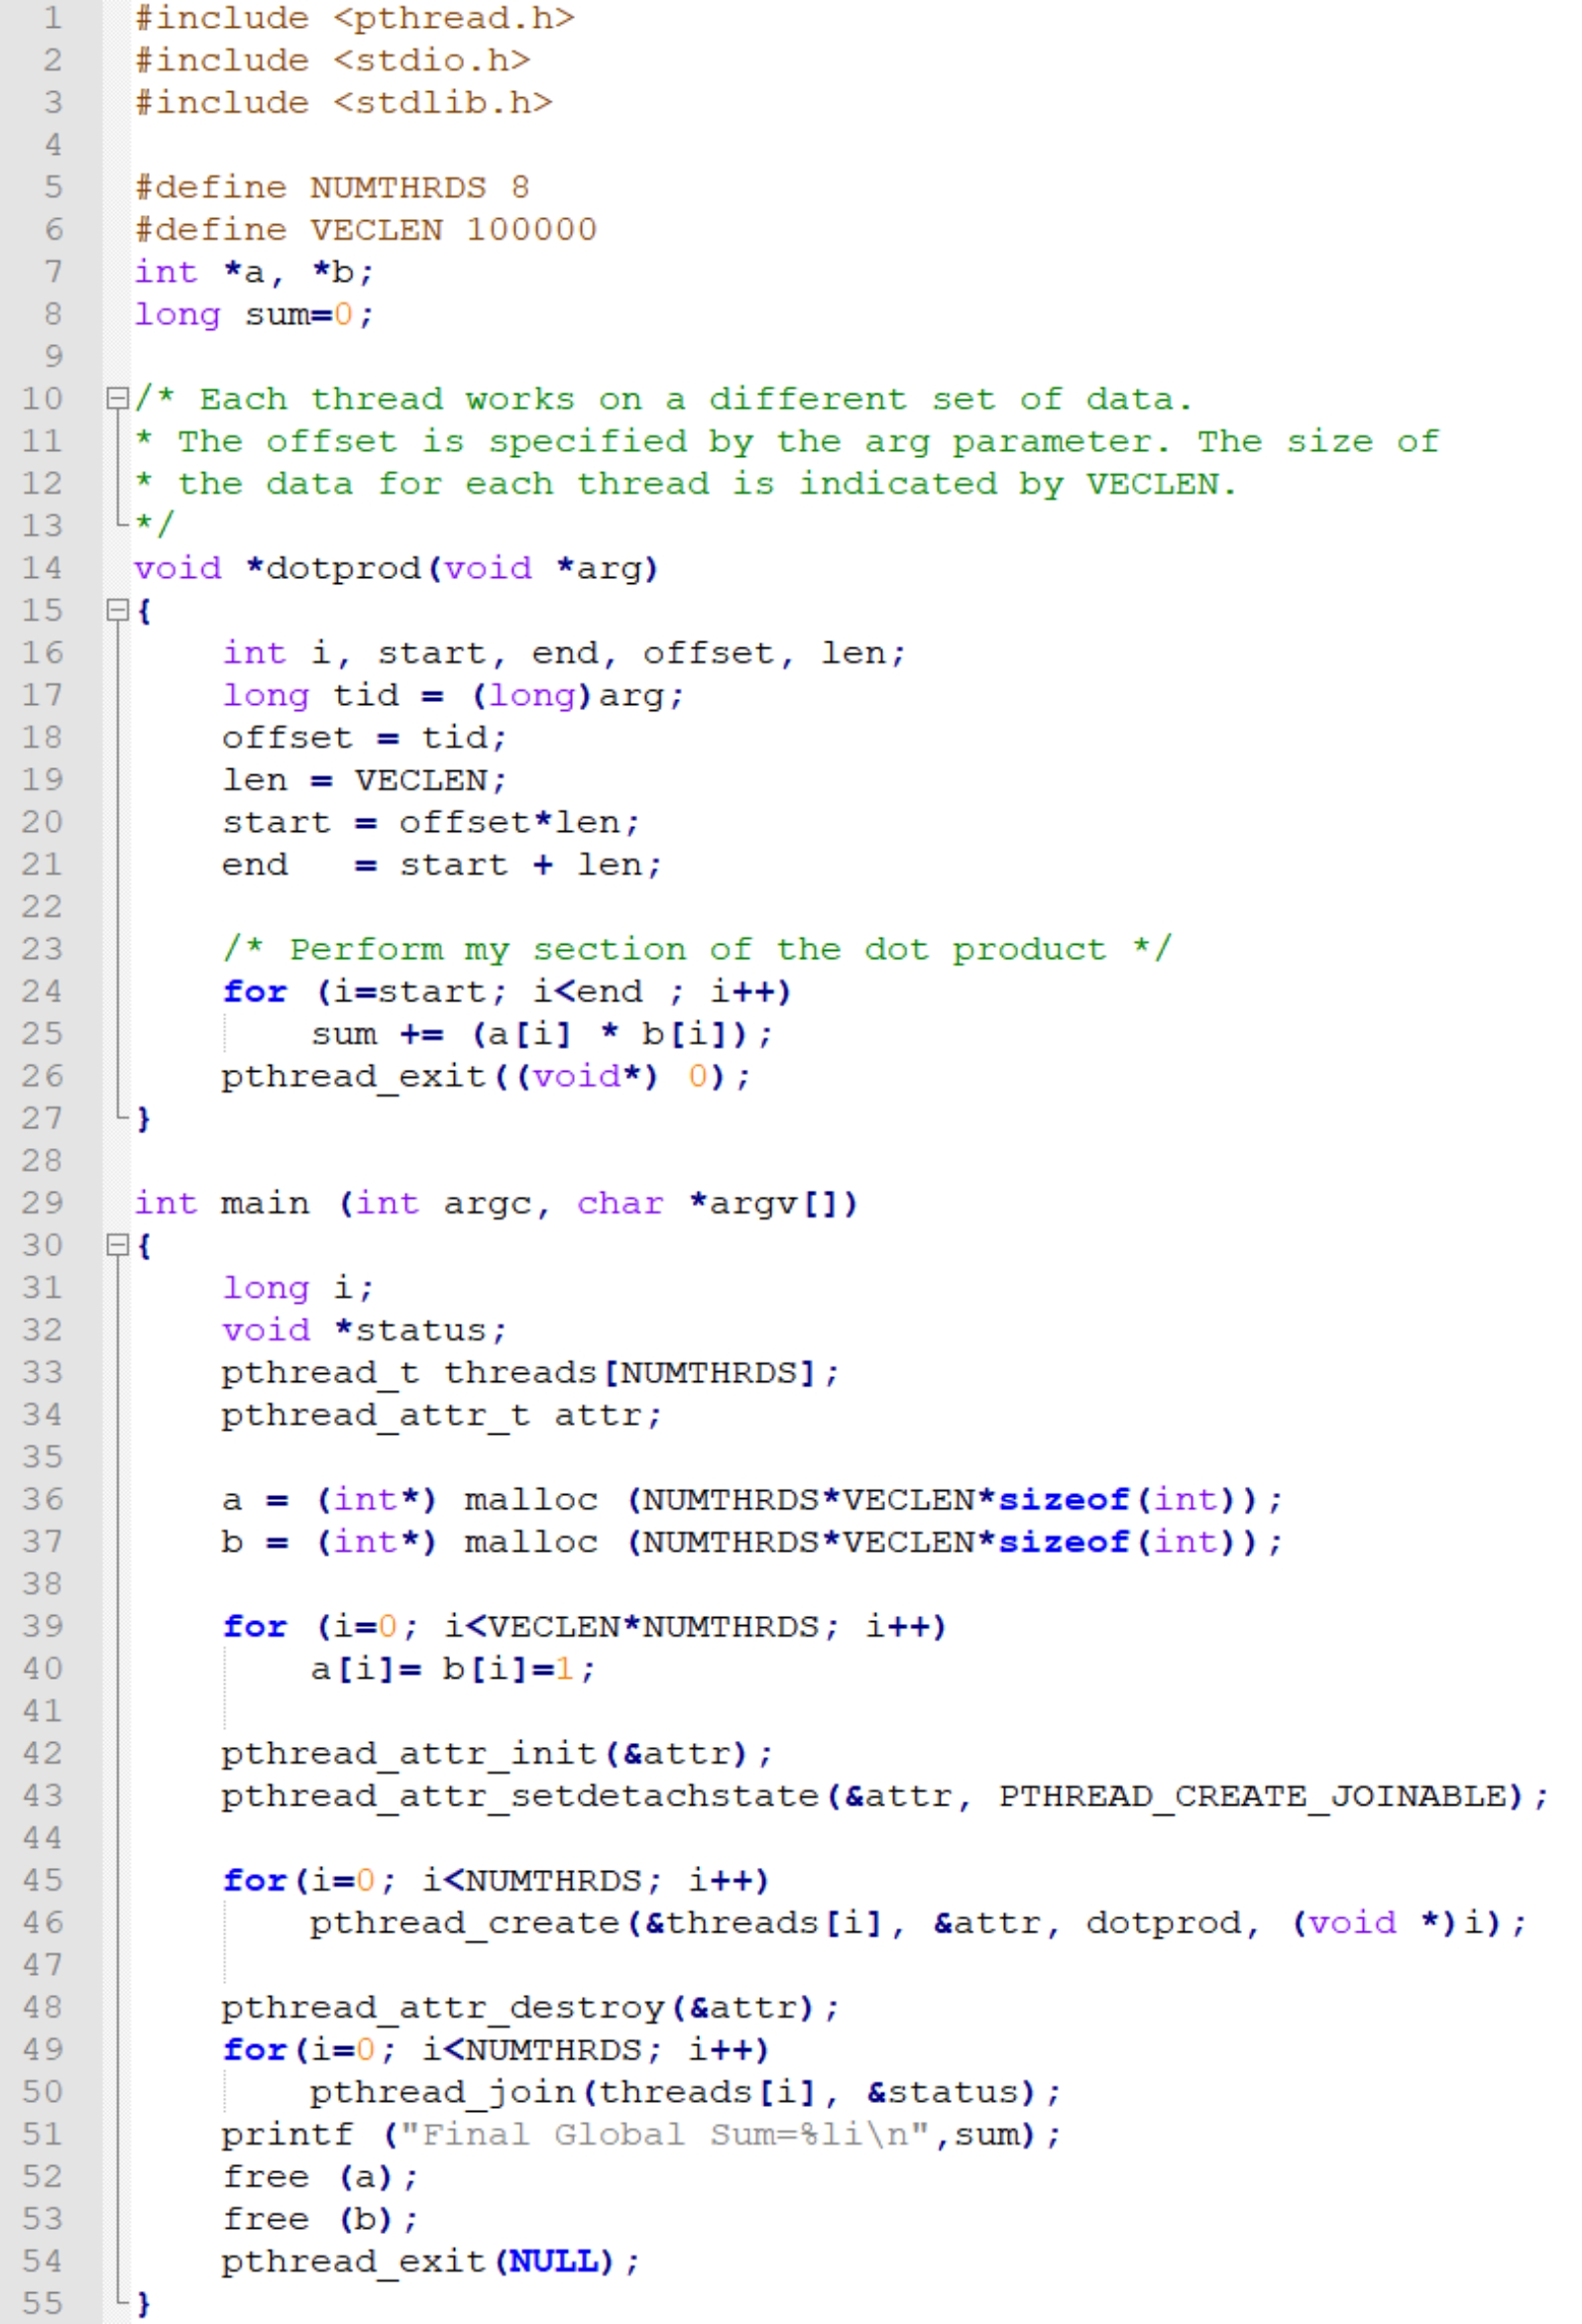
\includegraphics[width=4in]{q3code.jpg}
    \end{center}
    
    The code can be fixed by making the following changes. Assume all system
    calls succeed.
\begin{verbatim}
    // Insert this code after line 8
    pthread_mutex_t mutex;

    // Replaced lines 24 with the following code:
    pthread_mutex_lock(&mutex);
    sum += (a[i] * b[i]);
    pthread_mutex_unlock(&mutex);

    // Insert this code after like 34
    pthread_mutex_init(&mutex, NULL);
\end{verbatim}
\end{document}